% Created by tikzDevice version 0.12.3.1 on 2022-08-31 08:49:15
% !TEX encoding = UTF-8 Unicode
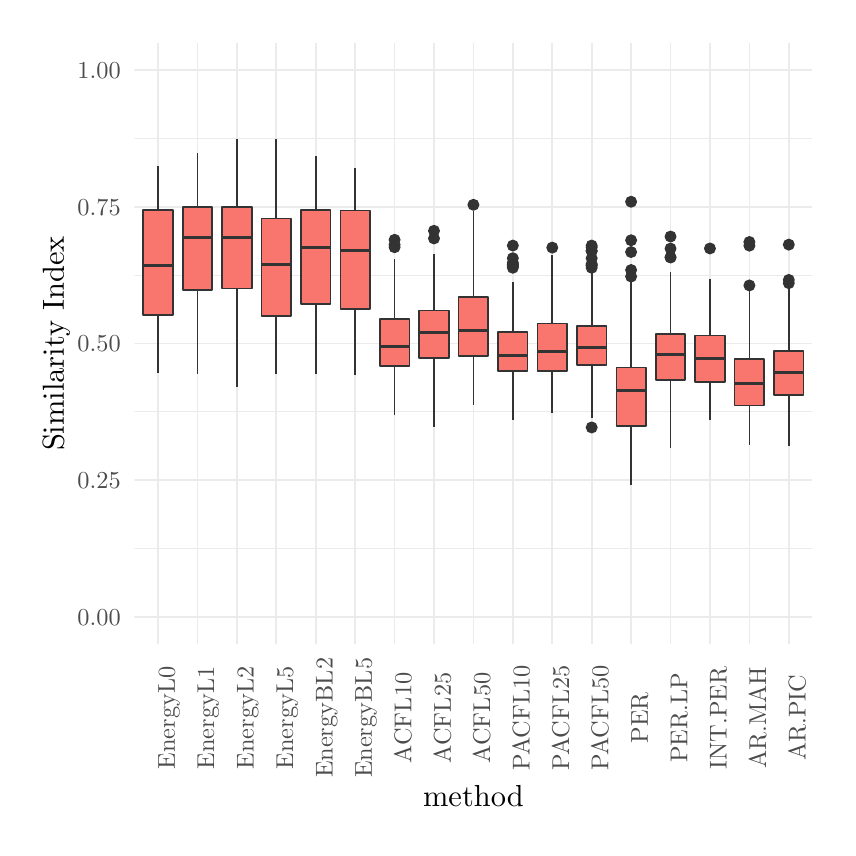
\begin{tikzpicture}[x=1pt,y=1pt]
\definecolor{fillColor}{RGB}{255,255,255}
\path[use as bounding box,fill=fillColor,fill opacity=0.00] (0,0) rectangle (289.08,289.08);
\begin{scope}
\path[clip] ( 38.56, 66.32) rectangle (283.58,283.58);
\definecolor{drawColor}{gray}{0.92}

\path[draw=drawColor,line width= 0.3pt,line join=round] ( 38.56,100.88) --
	(283.58,100.88);

\path[draw=drawColor,line width= 0.3pt,line join=round] ( 38.56,150.26) --
	(283.58,150.26);

\path[draw=drawColor,line width= 0.3pt,line join=round] ( 38.56,199.64) --
	(283.58,199.64);

\path[draw=drawColor,line width= 0.3pt,line join=round] ( 38.56,249.02) --
	(283.58,249.02);

\path[draw=drawColor,line width= 0.6pt,line join=round] ( 38.56, 76.19) --
	(283.58, 76.19);

\path[draw=drawColor,line width= 0.6pt,line join=round] ( 38.56,125.57) --
	(283.58,125.57);

\path[draw=drawColor,line width= 0.6pt,line join=round] ( 38.56,174.95) --
	(283.58,174.95);

\path[draw=drawColor,line width= 0.6pt,line join=round] ( 38.56,224.33) --
	(283.58,224.33);

\path[draw=drawColor,line width= 0.6pt,line join=round] ( 38.56,273.70) --
	(283.58,273.70);

\path[draw=drawColor,line width= 0.6pt,line join=round] ( 47.10, 66.32) --
	( 47.10,283.58);

\path[draw=drawColor,line width= 0.6pt,line join=round] ( 61.35, 66.32) --
	( 61.35,283.58);

\path[draw=drawColor,line width= 0.6pt,line join=round] ( 75.59, 66.32) --
	( 75.59,283.58);

\path[draw=drawColor,line width= 0.6pt,line join=round] ( 89.84, 66.32) --
	( 89.84,283.58);

\path[draw=drawColor,line width= 0.6pt,line join=round] (104.08, 66.32) --
	(104.08,283.58);

\path[draw=drawColor,line width= 0.6pt,line join=round] (118.33, 66.32) --
	(118.33,283.58);

\path[draw=drawColor,line width= 0.6pt,line join=round] (132.58, 66.32) --
	(132.58,283.58);

\path[draw=drawColor,line width= 0.6pt,line join=round] (146.82, 66.32) --
	(146.82,283.58);

\path[draw=drawColor,line width= 0.6pt,line join=round] (161.07, 66.32) --
	(161.07,283.58);

\path[draw=drawColor,line width= 0.6pt,line join=round] (175.31, 66.32) --
	(175.31,283.58);

\path[draw=drawColor,line width= 0.6pt,line join=round] (189.56, 66.32) --
	(189.56,283.58);

\path[draw=drawColor,line width= 0.6pt,line join=round] (203.80, 66.32) --
	(203.80,283.58);

\path[draw=drawColor,line width= 0.6pt,line join=round] (218.05, 66.32) --
	(218.05,283.58);

\path[draw=drawColor,line width= 0.6pt,line join=round] (232.30, 66.32) --
	(232.30,283.58);

\path[draw=drawColor,line width= 0.6pt,line join=round] (246.54, 66.32) --
	(246.54,283.58);

\path[draw=drawColor,line width= 0.6pt,line join=round] (260.79, 66.32) --
	(260.79,283.58);

\path[draw=drawColor,line width= 0.6pt,line join=round] (275.03, 66.32) --
	(275.03,283.58);
\definecolor{drawColor}{gray}{0.20}

\path[draw=drawColor,line width= 0.6pt,line join=round] ( 47.10,223.12) -- ( 47.10,239.05);

\path[draw=drawColor,line width= 0.6pt,line join=round] ( 47.10,185.23) -- ( 47.10,164.26);
\definecolor{fillColor}{RGB}{248,118,109}

\path[draw=drawColor,line width= 0.6pt,line join=round,line cap=round,fill=fillColor] ( 41.76,223.12) --
	( 41.76,185.23) --
	( 52.44,185.23) --
	( 52.44,223.12) --
	( 41.76,223.12) --
	cycle;

\path[draw=drawColor,line width= 1.1pt,line join=round] ( 41.76,203.27) -- ( 52.44,203.27);

\path[draw=drawColor,line width= 0.6pt,line join=round] ( 61.35,224.33) -- ( 61.35,243.78);

\path[draw=drawColor,line width= 0.6pt,line join=round] ( 61.35,194.32) -- ( 61.35,163.80);

\path[draw=drawColor,line width= 0.6pt,line join=round,line cap=round,fill=fillColor] ( 56.01,224.33) --
	( 56.01,194.32) --
	( 66.69,194.32) --
	( 66.69,224.33) --
	( 56.01,224.33) --
	cycle;

\path[draw=drawColor,line width= 1.1pt,line join=round] ( 56.01,213.24) -- ( 66.69,213.24);

\path[draw=drawColor,line width= 0.6pt,line join=round] ( 75.59,224.20) -- ( 75.59,248.95);

\path[draw=drawColor,line width= 0.6pt,line join=round] ( 75.59,194.83) -- ( 75.59,159.24);

\path[draw=drawColor,line width= 0.6pt,line join=round,line cap=round,fill=fillColor] ( 70.25,224.20) --
	( 70.25,194.83) --
	( 80.94,194.83) --
	( 80.94,224.20) --
	( 70.25,224.20) --
	cycle;

\path[draw=drawColor,line width= 1.1pt,line join=round] ( 70.25,213.23) -- ( 80.94,213.23);

\path[draw=drawColor,line width= 0.6pt,line join=round] ( 89.84,220.15) -- ( 89.84,248.95);

\path[draw=drawColor,line width= 0.6pt,line join=round] ( 89.84,184.83) -- ( 89.84,163.98);

\path[draw=drawColor,line width= 0.6pt,line join=round,line cap=round,fill=fillColor] ( 84.50,220.15) --
	( 84.50,184.83) --
	( 95.18,184.83) --
	( 95.18,220.15) --
	( 84.50,220.15) --
	cycle;

\path[draw=drawColor,line width= 1.1pt,line join=round] ( 84.50,203.59) -- ( 95.18,203.59);

\path[draw=drawColor,line width= 0.6pt,line join=round] (104.08,223.12) -- (104.08,242.84);

\path[draw=drawColor,line width= 0.6pt,line join=round] (104.08,189.23) -- (104.08,163.80);

\path[draw=drawColor,line width= 0.6pt,line join=round,line cap=round,fill=fillColor] ( 98.74,223.12) --
	( 98.74,189.23) --
	(109.43,189.23) --
	(109.43,223.12) --
	( 98.74,223.12) --
	cycle;

\path[draw=drawColor,line width= 1.1pt,line join=round] ( 98.74,209.61) -- (109.43,209.61);

\path[draw=drawColor,line width= 0.6pt,line join=round] (118.33,223.06) -- (118.33,238.34);

\path[draw=drawColor,line width= 0.6pt,line join=round] (118.33,187.50) -- (118.33,163.49);

\path[draw=drawColor,line width= 0.6pt,line join=round,line cap=round,fill=fillColor] (112.99,223.06) --
	(112.99,187.50) --
	(123.67,187.50) --
	(123.67,223.06) --
	(112.99,223.06) --
	cycle;

\path[draw=drawColor,line width= 1.1pt,line join=round] (112.99,208.67) -- (123.67,208.67);
\definecolor{fillColor}{gray}{0.20}

\path[draw=drawColor,line width= 0.4pt,line join=round,line cap=round,fill=fillColor] (132.58,210.68) circle (  1.96);

\path[draw=drawColor,line width= 0.4pt,line join=round,line cap=round,fill=fillColor] (132.58,209.74) circle (  1.96);

\path[draw=drawColor,line width= 0.4pt,line join=round,line cap=round,fill=fillColor] (132.58,212.42) circle (  1.96);

\path[draw=drawColor,line width= 0.6pt,line join=round] (132.58,183.89) -- (132.58,205.46);

\path[draw=drawColor,line width= 0.6pt,line join=round] (132.58,166.93) -- (132.58,149.01);
\definecolor{fillColor}{RGB}{248,118,109}

\path[draw=drawColor,line width= 0.6pt,line join=round,line cap=round,fill=fillColor] (127.23,183.89) --
	(127.23,166.93) --
	(137.92,166.93) --
	(137.92,183.89) --
	(127.23,183.89) --
	cycle;

\path[draw=drawColor,line width= 1.1pt,line join=round] (127.23,173.85) -- (137.92,173.85);
\definecolor{fillColor}{gray}{0.20}

\path[draw=drawColor,line width= 0.4pt,line join=round,line cap=round,fill=fillColor] (146.82,215.67) circle (  1.96);

\path[draw=drawColor,line width= 0.4pt,line join=round,line cap=round,fill=fillColor] (146.82,212.92) circle (  1.96);

\path[draw=drawColor,line width= 0.6pt,line join=round] (146.82,186.86) -- (146.82,207.20);

\path[draw=drawColor,line width= 0.6pt,line join=round] (146.82,169.68) -- (146.82,144.64);
\definecolor{fillColor}{RGB}{248,118,109}

\path[draw=drawColor,line width= 0.6pt,line join=round,line cap=round,fill=fillColor] (141.48,186.86) --
	(141.48,169.68) --
	(152.16,169.68) --
	(152.16,186.86) --
	(141.48,186.86) --
	cycle;

\path[draw=drawColor,line width= 1.1pt,line join=round] (141.48,179.03) -- (152.16,179.03);
\definecolor{fillColor}{gray}{0.20}

\path[draw=drawColor,line width= 0.4pt,line join=round,line cap=round,fill=fillColor] (161.07,225.08) circle (  1.96);

\path[draw=drawColor,line width= 0.6pt,line join=round] (161.07,191.68) -- (161.07,223.00);

\path[draw=drawColor,line width= 0.6pt,line join=round] (161.07,170.42) -- (161.07,152.70);
\definecolor{fillColor}{RGB}{248,118,109}

\path[draw=drawColor,line width= 0.6pt,line join=round,line cap=round,fill=fillColor] (155.73,191.68) --
	(155.73,170.42) --
	(166.41,170.42) --
	(166.41,191.68) --
	(155.73,191.68) --
	cycle;

\path[draw=drawColor,line width= 1.1pt,line join=round] (155.73,179.78) -- (166.41,179.78);
\definecolor{fillColor}{gray}{0.20}

\path[draw=drawColor,line width= 0.4pt,line join=round,line cap=round,fill=fillColor] (175.31,203.08) circle (  1.96);

\path[draw=drawColor,line width= 0.4pt,line join=round,line cap=round,fill=fillColor] (175.31,203.56) circle (  1.96);

\path[draw=drawColor,line width= 0.4pt,line join=round,line cap=round,fill=fillColor] (175.31,210.34) circle (  1.96);

\path[draw=drawColor,line width= 0.4pt,line join=round,line cap=round,fill=fillColor] (175.31,205.77) circle (  1.96);

\path[draw=drawColor,line width= 0.4pt,line join=round,line cap=round,fill=fillColor] (175.31,202.32) circle (  1.96);

\path[draw=drawColor,line width= 0.4pt,line join=round,line cap=round,fill=fillColor] (175.31,204.11) circle (  1.96);

\path[draw=drawColor,line width= 0.4pt,line join=round,line cap=round,fill=fillColor] (175.31,202.95) circle (  1.96);

\path[draw=drawColor,line width= 0.6pt,line join=round] (175.31,179.11) -- (175.31,197.23);

\path[draw=drawColor,line width= 0.6pt,line join=round] (175.31,164.92) -- (175.31,147.19);
\definecolor{fillColor}{RGB}{248,118,109}

\path[draw=drawColor,line width= 0.6pt,line join=round,line cap=round,fill=fillColor] (169.97,179.11) --
	(169.97,164.92) --
	(180.66,164.92) --
	(180.66,179.11) --
	(169.97,179.11) --
	cycle;

\path[draw=drawColor,line width= 1.1pt,line join=round] (169.97,170.63) -- (180.66,170.63);
\definecolor{fillColor}{gray}{0.20}

\path[draw=drawColor,line width= 0.4pt,line join=round,line cap=round,fill=fillColor] (189.56,209.60) circle (  1.96);

\path[draw=drawColor,line width= 0.6pt,line join=round] (189.56,182.13) -- (189.56,206.81);

\path[draw=drawColor,line width= 0.6pt,line join=round] (189.56,164.91) -- (189.56,150.02);
\definecolor{fillColor}{RGB}{248,118,109}

\path[draw=drawColor,line width= 0.6pt,line join=round,line cap=round,fill=fillColor] (184.22,182.13) --
	(184.22,164.91) --
	(194.90,164.91) --
	(194.90,182.13) --
	(184.22,182.13) --
	cycle;

\path[draw=drawColor,line width= 1.1pt,line join=round] (184.22,172.03) -- (194.90,172.03);
\definecolor{fillColor}{gray}{0.20}

\path[draw=drawColor,line width= 0.4pt,line join=round,line cap=round,fill=fillColor] (203.80,205.75) circle (  1.96);

\path[draw=drawColor,line width= 0.4pt,line join=round,line cap=round,fill=fillColor] (203.80,203.20) circle (  1.96);

\path[draw=drawColor,line width= 0.4pt,line join=round,line cap=round,fill=fillColor] (203.80,203.70) circle (  1.96);

\path[draw=drawColor,line width= 0.4pt,line join=round,line cap=round,fill=fillColor] (203.80,210.34) circle (  1.96);

\path[draw=drawColor,line width= 0.4pt,line join=round,line cap=round,fill=fillColor] (203.80,208.39) circle (  1.96);

\path[draw=drawColor,line width= 0.4pt,line join=round,line cap=round,fill=fillColor] (203.80,202.32) circle (  1.96);

\path[draw=drawColor,line width= 0.4pt,line join=round,line cap=round,fill=fillColor] (203.80,144.62) circle (  1.96);

\path[draw=drawColor,line width= 0.4pt,line join=round,line cap=round,fill=fillColor] (203.80,208.39) circle (  1.96);

\path[draw=drawColor,line width= 0.4pt,line join=round,line cap=round,fill=fillColor] (203.80,209.66) circle (  1.96);

\path[draw=drawColor,line width= 0.4pt,line join=round,line cap=round,fill=fillColor] (203.80,203.19) circle (  1.96);

\path[draw=drawColor,line width= 0.6pt,line join=round] (203.80,181.25) -- (203.80,201.06);

\path[draw=drawColor,line width= 0.6pt,line join=round] (203.80,167.23) -- (203.80,148.06);
\definecolor{fillColor}{RGB}{248,118,109}

\path[draw=drawColor,line width= 0.6pt,line join=round,line cap=round,fill=fillColor] (198.46,181.25) --
	(198.46,167.23) --
	(209.15,167.23) --
	(209.15,181.25) --
	(198.46,181.25) --
	cycle;

\path[draw=drawColor,line width= 1.1pt,line join=round] (198.46,173.62) -- (209.15,173.62);
\definecolor{fillColor}{gray}{0.20}

\path[draw=drawColor,line width= 0.4pt,line join=round,line cap=round,fill=fillColor] (218.05,199.15) circle (  1.96);

\path[draw=drawColor,line width= 0.4pt,line join=round,line cap=round,fill=fillColor] (218.05,208.00) circle (  1.96);

\path[draw=drawColor,line width= 0.4pt,line join=round,line cap=round,fill=fillColor] (218.05,212.26) circle (  1.96);

\path[draw=drawColor,line width= 0.4pt,line join=round,line cap=round,fill=fillColor] (218.05,201.51) circle (  1.96);

\path[draw=drawColor,line width= 0.4pt,line join=round,line cap=round,fill=fillColor] (218.05,226.18) circle (  1.96);

\path[draw=drawColor,line width= 0.6pt,line join=round] (218.05,166.25) -- (218.05,197.65);

\path[draw=drawColor,line width= 0.6pt,line join=round] (218.05,145.26) -- (218.05,123.85);
\definecolor{fillColor}{RGB}{248,118,109}

\path[draw=drawColor,line width= 0.6pt,line join=round,line cap=round,fill=fillColor] (212.71,166.25) --
	(212.71,145.26) --
	(223.39,145.26) --
	(223.39,166.25) --
	(212.71,166.25) --
	cycle;

\path[draw=drawColor,line width= 1.1pt,line join=round] (212.71,157.99) -- (223.39,157.99);
\definecolor{fillColor}{gray}{0.20}

\path[draw=drawColor,line width= 0.4pt,line join=round,line cap=round,fill=fillColor] (232.30,209.26) circle (  1.96);

\path[draw=drawColor,line width= 0.4pt,line join=round,line cap=round,fill=fillColor] (232.30,213.60) circle (  1.96);

\path[draw=drawColor,line width= 0.4pt,line join=round,line cap=round,fill=fillColor] (232.30,206.06) circle (  1.96);

\path[draw=drawColor,line width= 0.4pt,line join=round,line cap=round,fill=fillColor] (232.30,206.10) circle (  1.96);

\path[draw=drawColor,line width= 0.6pt,line join=round] (232.30,178.41) -- (232.30,200.61);

\path[draw=drawColor,line width= 0.6pt,line join=round] (232.30,161.79) -- (232.30,137.27);
\definecolor{fillColor}{RGB}{248,118,109}

\path[draw=drawColor,line width= 0.6pt,line join=round,line cap=round,fill=fillColor] (226.95,178.41) --
	(226.95,161.79) --
	(237.64,161.79) --
	(237.64,178.41) --
	(226.95,178.41) --
	cycle;

\path[draw=drawColor,line width= 1.1pt,line join=round] (226.95,170.87) -- (237.64,170.87);
\definecolor{fillColor}{gray}{0.20}

\path[draw=drawColor,line width= 0.4pt,line join=round,line cap=round,fill=fillColor] (246.54,209.30) circle (  1.96);

\path[draw=drawColor,line width= 0.6pt,line join=round] (246.54,177.89) -- (246.54,198.35);

\path[draw=drawColor,line width= 0.6pt,line join=round] (246.54,161.06) -- (246.54,147.37);
\definecolor{fillColor}{RGB}{248,118,109}

\path[draw=drawColor,line width= 0.6pt,line join=round,line cap=round,fill=fillColor] (241.20,177.89) --
	(241.20,161.06) --
	(251.88,161.06) --
	(251.88,177.89) --
	(241.20,177.89) --
	cycle;

\path[draw=drawColor,line width= 1.1pt,line join=round] (241.20,169.70) -- (251.88,169.70);
\definecolor{fillColor}{gray}{0.20}

\path[draw=drawColor,line width= 0.4pt,line join=round,line cap=round,fill=fillColor] (260.79,195.94) circle (  1.96);

\path[draw=drawColor,line width= 0.4pt,line join=round,line cap=round,fill=fillColor] (260.79,211.63) circle (  1.96);

\path[draw=drawColor,line width= 0.4pt,line join=round,line cap=round,fill=fillColor] (260.79,210.31) circle (  1.96);

\path[draw=drawColor,line width= 0.6pt,line join=round] (260.79,169.46) -- (260.79,194.85);

\path[draw=drawColor,line width= 0.6pt,line join=round] (260.79,152.49) -- (260.79,138.35);
\definecolor{fillColor}{RGB}{248,118,109}

\path[draw=drawColor,line width= 0.6pt,line join=round,line cap=round,fill=fillColor] (255.44,169.46) --
	(255.44,152.49) --
	(266.13,152.49) --
	(266.13,169.46) --
	(255.44,169.46) --
	cycle;

\path[draw=drawColor,line width= 1.1pt,line join=round] (255.44,160.47) -- (266.13,160.47);
\definecolor{fillColor}{gray}{0.20}

\path[draw=drawColor,line width= 0.4pt,line join=round,line cap=round,fill=fillColor] (275.03,210.68) circle (  1.96);

\path[draw=drawColor,line width= 0.4pt,line join=round,line cap=round,fill=fillColor] (275.03,197.93) circle (  1.96);

\path[draw=drawColor,line width= 0.4pt,line join=round,line cap=round,fill=fillColor] (275.03,196.76) circle (  1.96);

\path[draw=drawColor,line width= 0.6pt,line join=round] (275.03,172.32) -- (275.03,195.94);

\path[draw=drawColor,line width= 0.6pt,line join=round] (275.03,156.31) -- (275.03,138.02);
\definecolor{fillColor}{RGB}{248,118,109}

\path[draw=drawColor,line width= 0.6pt,line join=round,line cap=round,fill=fillColor] (269.69,172.32) --
	(269.69,156.31) --
	(280.37,156.31) --
	(280.37,172.32) --
	(269.69,172.32) --
	cycle;

\path[draw=drawColor,line width= 1.1pt,line join=round] (269.69,164.64) -- (280.37,164.64);
\end{scope}
\begin{scope}
\path[clip] (  0.00,  0.00) rectangle (289.08,289.08);
\definecolor{drawColor}{gray}{0.30}

\node[text=drawColor,anchor=base east,inner sep=0pt, outer sep=0pt, scale=  0.88] at ( 33.61, 73.16) {0.00};

\node[text=drawColor,anchor=base east,inner sep=0pt, outer sep=0pt, scale=  0.88] at ( 33.61,122.54) {0.25};

\node[text=drawColor,anchor=base east,inner sep=0pt, outer sep=0pt, scale=  0.88] at ( 33.61,171.92) {0.50};

\node[text=drawColor,anchor=base east,inner sep=0pt, outer sep=0pt, scale=  0.88] at ( 33.61,221.30) {0.75};

\node[text=drawColor,anchor=base east,inner sep=0pt, outer sep=0pt, scale=  0.88] at ( 33.61,270.67) {1.00};
\end{scope}
\begin{scope}
\path[clip] (  0.00,  0.00) rectangle (289.08,289.08);
\definecolor{drawColor}{gray}{0.30}

\node[text=drawColor,rotate= 90.00,anchor=base,inner sep=0pt, outer sep=0pt, scale=  0.88] at ( 53.16, 39.67) {EnergyL0};

\node[text=drawColor,rotate= 90.00,anchor=base,inner sep=0pt, outer sep=0pt, scale=  0.88] at ( 67.41, 39.67) {EnergyL1};

\node[text=drawColor,rotate= 90.00,anchor=base,inner sep=0pt, outer sep=0pt, scale=  0.88] at ( 81.65, 39.67) {EnergyL2};

\node[text=drawColor,rotate= 90.00,anchor=base,inner sep=0pt, outer sep=0pt, scale=  0.88] at ( 95.90, 39.67) {EnergyL5};

\node[text=drawColor,rotate= 90.00,anchor=base,inner sep=0pt, outer sep=0pt, scale=  0.88] at (110.15, 39.67) {EnergyBL2};

\node[text=drawColor,rotate= 90.00,anchor=base,inner sep=0pt, outer sep=0pt, scale=  0.88] at (124.39, 39.67) {EnergyBL5};

\node[text=drawColor,rotate= 90.00,anchor=base,inner sep=0pt, outer sep=0pt, scale=  0.88] at (138.64, 39.67) {ACFL10};

\node[text=drawColor,rotate= 90.00,anchor=base,inner sep=0pt, outer sep=0pt, scale=  0.88] at (152.88, 39.67) {ACFL25};

\node[text=drawColor,rotate= 90.00,anchor=base,inner sep=0pt, outer sep=0pt, scale=  0.88] at (167.13, 39.67) {ACFL50};

\node[text=drawColor,rotate= 90.00,anchor=base,inner sep=0pt, outer sep=0pt, scale=  0.88] at (181.37, 39.67) {PACFL10};

\node[text=drawColor,rotate= 90.00,anchor=base,inner sep=0pt, outer sep=0pt, scale=  0.88] at (195.62, 39.67) {PACFL25};

\node[text=drawColor,rotate= 90.00,anchor=base,inner sep=0pt, outer sep=0pt, scale=  0.88] at (209.87, 39.67) {PACFL50};

\node[text=drawColor,rotate= 90.00,anchor=base,inner sep=0pt, outer sep=0pt, scale=  0.88] at (224.11, 39.67) {PER};

\node[text=drawColor,rotate= 90.00,anchor=base,inner sep=0pt, outer sep=0pt, scale=  0.88] at (238.36, 39.67) {PER.LP};

\node[text=drawColor,rotate= 90.00,anchor=base,inner sep=0pt, outer sep=0pt, scale=  0.88] at (252.60, 39.67) {INT.PER};

\node[text=drawColor,rotate= 90.00,anchor=base,inner sep=0pt, outer sep=0pt, scale=  0.88] at (266.85, 39.67) {AR.MAH};

\node[text=drawColor,rotate= 90.00,anchor=base,inner sep=0pt, outer sep=0pt, scale=  0.88] at (281.09, 39.67) {AR.PIC};
\end{scope}
\begin{scope}
\path[clip] (  0.00,  0.00) rectangle (289.08,289.08);
\definecolor{drawColor}{RGB}{0,0,0}

\node[text=drawColor,anchor=base,inner sep=0pt, outer sep=0pt, scale=  1.10] at (161.07,  7.64) {method};
\end{scope}
\begin{scope}
\path[clip] (  0.00,  0.00) rectangle (289.08,289.08);
\definecolor{drawColor}{RGB}{0,0,0}

\node[text=drawColor,rotate= 90.00,anchor=base,inner sep=0pt, outer sep=0pt, scale=  1.10] at ( 13.08,174.95) {Similarity Index};
\end{scope}
\end{tikzpicture}
